%!TEX TS-program = xelatex
%!TEX encoding = UTF-8 Unicode

\documentclass[a4paper, titlepage, 10pt, bookmark]{article}
\usepackage{geometry}
\usepackage{graphicx} 
\usepackage{listings}
\usepackage{xcolor}
\usepackage{setspace}
\usepackage{fontspec,xltxtra,xunicode}
\usepackage{titlesec}

%\usepackage[dvipdfm]{hyperref}

%\geometry{letterpaper}

\defaultfontfeatures{Mapping=tex-text}
\setromanfont{SimSun} %设置中文字体
\usepackage{fontspec}
\setmainfont{微软雅黑}

\linespread{1.2}

\XeTeXlinebreaklocale “zh”
\XeTeXlinebreakskip = 0pt plus 1pt minus 0.1pt %文章内中文自动换行

\definecolor{sectionblue}{rgb}{0.37, 0.72, 0.99}
\titleformat{\section}
	{\color{sectionblue}\normalfont\Large\bfseries}
	{\color{sectionblue}\thesection}{1em}{}

\titleformat{\subsection}
	{\color{sectionblue}\normalfont\large\bfseries}
	{\color{sectionblue}\thesubsection}{1em}{}

\titleformat{\subsubsection}
	{\color{sectionblue}\normalfont\large\bfseries}
	{\color{sectionblue}\thesubsubsection}{1em}{}

%%%% --begin: 设置lstlisting
\definecolor{dkgreen}{rgb}{0, 0.6, 0}
\definecolor{gray}{rgb}{0.5, 0.5, 0.5}
\definecolor{darkgray}{rgb}{0.4, 0.4, 0.4}
\definecolor{lightgray}{rgb}{0.99, 0.99, 0.99}
\definecolor{mauve}{rgb}{0.58, 0, 0.82}

\lstset{
  backgroundcolor=\color{lightgray}, % choose the background color
  basicstyle=\scriptsize,         % the size of the fonts for the code
  %breakatwhitespace=false,       % breaks should only happen at whitespace
  breaklines=true,                % sets automatic line breaking
  captionpos=b,                   % sets the caption-position to bottom
  commentstyle=\color{dkgreen},   % comment style
  %deletekeywords={...},          %  delete keywords from the given language
  %escapeinside={\%*}{*)},        % if you want to add LaTeX within your code
  %extendedchar=true,             % lets you use non-ASCII characters; for 8-bits encodings only, does not work with UTF-8
  frame=single,                   % adds a frame around the code
  keywordstyle=\color{blue},      % keyword style
  language=Java,                  % the language of the code
  morekeywords={val,def,object},  % add more keywords to the set
  %numbers=left,                  % where to put the line-numbers; possible values are (none, left, right)
  %numbersep=5pt,                  % how far the line-numbers are from the code
  %numberstyle=\tiny\color{gray},  % the style that is used for the line-numbers
  rulecolor=\color{black},        % if not set, the frame-color may be changed on line-breaks within not-black text (e.g. comments (green here))
  showspaces=false,               % show spaces everywhere adding particular underscores; it overrides 'showstringspaces'
  showstringspaces=false,         % underline spaces within strings only
  showtabs=false,                 % show tabs within strings adding particular underscores
  %stepnumber=2,                   % the step between two line-numbers. If it's 1, each line will be numbered
  stringstyle=\color{mauve},      % string literal style
  tabsize=4,                      % sets default tabsize to 2 spaces
  % title=\lstname                  % show the filename of files included with \lstinputlisting; also try caption instead of title
}

%%%% --end

\usepackage[unicode]{hyperref}
\setlength{\parindent}{0pt}
\graphicspath{{images/}}

\newfontfamily{\H}{SimHei}
\newfontfamily{\E}{Arial}
\title{\H \color{gray}MySQL协议文档}
\author{\color{gray}Alex Wang}
\date{\E\color{gray}\today}

\begin{document}
\setcounter{secnumdepth}{6}
\setcounter{tocdepth}{5}
\maketitle

\color{darkgray}
\tableofcontents
\newpage








\section{概述}
MySQL协议用于MySQL客户端与服务器端的交互。MySQL Connectors库(包括Connector/C、Connector/J等等)、MySQL Proxy、以及MySQL复制方案中Master和Slave之间都使用MySQL协议。\\

MySQL协议支持以下特性:
\begin{itemize}
    \item 使用SSL透明加密
    \item MySQL Server能力和认证数据交换
    \item 支持SQL语句的预编译以及存储过程的调用
\end{itemize}

本文档基于以下的源代码:
\begin{itemize}
    \item sql/sql\_parse.cc文件中的基础协议函数:dispatch\_command()
    \item sql/sql\_prepare.cc文件中的SQL预编译相关协议处理函数:mysqld
    \_stmt\_prepare()、mysqld\_stmt\_execute()、mysqld\_stmt\_close()、mysqld\_stmt\_reset()、mysqld\_stmt\_fetch()、mysql\_stmt\_get\_longdata() 
    \item sql/sql\_repl.cc文件中的binlog处理函数:mysql\_binlog\_send()
    \item sql/protocol.cc文件中关于类型和值编码的部分
\end{itemize}

\subsection{基础类型}
\subsubsection{整数类型}
MySQL协议包含了两种整数类型编码方式:
\begin{itemize}
    \item 定长整数
    \item 变长(length-encoded)整数
\end{itemize}

\paragraph{定长整数}
定长整数类型(Protocol::FixedLengthInteger)包括了type 1、type 2、type 3、type 4、type 6、type 8共六种长度的整数。在存储的时候,低位在前,比如,type 3类型的1存储为:
\begin{spacing}{1.0}
\begin{lstlisting}
01 00 00
\end{lstlisting}
\end{spacing}

\paragraph{变长整数}
变长整数类型(Protocol::LengthEncodedInteger)根据值的大小长度可能是1、3、4或者9个byte。变长整数的编码方式如下:
\begin{itemize}
    \item 如果value < 251,使用1 byte
    \item 如果value >= 251 同时 value < 2 ** 16,使用fc + 2 byte
    \item 如果value >= 2 ** 16 同时 value < 2 ** 24,使用fd + 3 byte
    \item 如果value >= 2 ** 24 同时 value < 2 ** 64,使用fe + 8 byte
\end{itemize}

当需要获取变长整数的值时只需要先检查第一个byte,然后判断长度:
\begin{itemize}
    \item 如果第一个byte位 < 251,转换为1byte的整数
    \item 如果第一个byte位 >= 251 同时 < 2 ** 16,则将后两位转换为2 byte的整数
    \item 如果第一个byte位 >= 2 ** 16 同时 < 2 ** 24,则将后三位转换为3 byte的整数
    \item 如果第一个byte位 >= 2 ** 24 同时 < 2 ** 64,则将后八位转换为8 byte的整数
\end{itemize}

下面章节使用lenenc\_int表示变长整数。

\subsubsection{String类型}
String类型是一个byte数组,在协议中可以有以下的编码方式:
\begin{itemize}
    \item Protocol::FixedLengthString:长度已知的字符串,比如ERR\_Packet包中的sql-state字段的长度总是5,以下简称string.fix\_len
    \item Protocol::NulTerminatedString:以[00]结尾的字符串,以下简称string.NUL
    \item Protocol::VariableLengthString:字符串的长度由其它字段表示、或者在运行时计算得出,以下简称string.var\_len
    \item Protocol::LengthEncodedString:字符串有一个变长整型的前缀表示其长度,是Protocol::VariableLengthString的一个特例,以下简称lenenc\_str
    \item Protocol::RestOfPacketString:字符串位于一个包的尾部,它的长度可由包的长度减去当前位置获取,以下简称string.EOF
\end{itemize}



\subsection{MySQL包}
当MySQL客户端或者服务器端发送数据时,必须:
\begin{itemize}
    \item 将数据切分成长度不超过$2^{24}$-1,那么持续发送长度为(0xffffff)的包,直到包的长度小于$2^{24}$-1。的数据包
    \item 为每个数据包添加一个包头
\end{itemize}

下图表示一个超长包的打包示意图:
\begin{center}
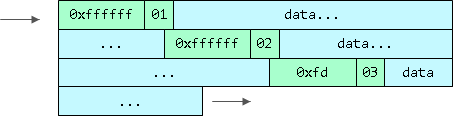
\includegraphics[width=4in]{027.png}
\end{center}

MySQL数据包长度不超过16MB,每个包包含以下内容:
\begin{itemize}
    \item 3 byte:      包体长度,不包含4个byte的头
    \item 1 byte:      序列号
    \item string[len]: 包体内容
\end{itemize}

比如COM\_QUIT的编码如下:
\begin{spacing}{1.0}
\begin{lstlisting}
01 00 00 00 01  /* length=0x01, sequence id=0x01, command=0x01*/
\end{lstlisting}
\end{spacing}

\subsubsection{大于16MB的包}
如果发送的数据长度大于$2^{24}$-1,那么持续发送长度为(0xffffff)的包,直到包的长度小于$2^{24}$-1。

\subsubsection{序列号}
在一个命令交互过程中,序列号从0开始,每个包递增1;当处理下一个命令序列时,清零。



\subsection{通用响应包}
对于大多数客户端发出的命令,服务器端响应OR\_Packet、 ERR\_Packet或EOF\_Packet。

\subsubsection{OR\_Packet}
MySQL服务器发送OK包表示命令处理成功。如果设置了CLIENT\_PROTOCOL\_41,OK包中包含一个warning数量的字段。OK包的格式描述如下:
\begin{spacing}{1.0}
\begin{lstlisting}
1              [00] the OK header
lenenc-int     affected rows
lenenc-int     last-insert-id
//if capabilities & CLIENT_PROTOCOL_41 {
2              status_flags
2              warnings
//} elseif capabilities & CLIENT_TRANSACTIONS {
2              status_flags
//}
// if capabilities & CLIENT_SESSION_TRACK {
lenenc-str     info
    // if n > 0 {
lenenc-int     total length (n) of session state-change
               information to follow
n              session state-change information
    //}
//}
// else {
string[EOF]    info
// }
\end{lstlisting}
\end{spacing}

[TODO] 字段解释

\subsubsection{ERR\_Packet}
表示MySQL Server处理命令时发生错误,格式如下:
\begin{spacing}{1.0}
\begin{lstlisting}
1              [ff] the ERR header
2              error code
// if capabilities & CLIENT_PROTOCOL_41 {
string[1]      '#' the sql-state marker
string[5]      sql-state
// }
string[EOF]    error-message
\end{lstlisting}
\end{spacing}

[TODO] 字段解释

\subsubsection{EOF\_Packet}
如果设置了CLIENT\_PROTOCOL\_41,EOF包会包含warning count和status flags字段:
\begin{spacing}{1.0}
\begin{lstlisting}
1              [fe] the EOF header
// if capabilities & CLIENT_PROTOCOL_41 {
2              warning count
2              status flags
// }
\end{lstlisting}
\end{spacing}

注意:EOF包可能会和Protocol::LengthEncodedInteger发生混淆,因此,必须通过检查包的长度是否小于9来确认是EOF包。

[TODO] 字段解释

\subsubsection{状态信息}
Protocol::StatusFlags取值如下:
\begin{center}
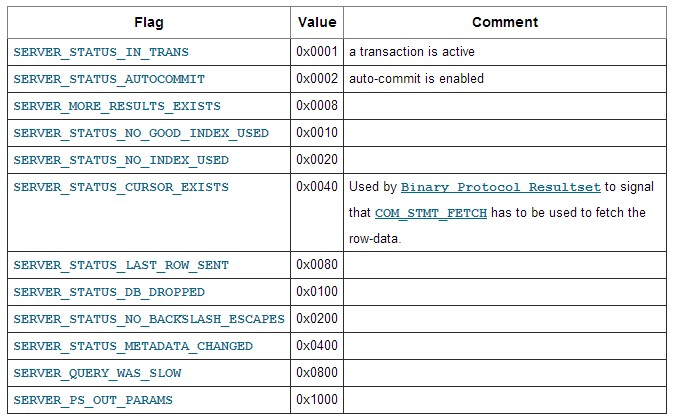
\includegraphics[width=7in]{001.jpg}
\end{center}



\subsection{连接的生命周期}
本节描述MySQL客户端和服务器连接的生命周期包括了连接建立阶段和命令处理阶段两个部分。下一章我们结合这两个阶段对MySQL协议处理过程进行详细描述。

\newpage









\section{连接建立}
连接建立阶段包括了:
\begin{itemize}
    \item 交换客户端和服务器端的能力
    \item 如果需要,建立SSL通道
    \item 对客户端进行认证
\end{itemize}

连接建立过程由客户端发起。当客户端同MySQL Server建立连接网络连接后,MySQL Server可以发送一个ERR\_Packet作为响应结束握手、或者发送一个Protocol::Handshake(握手包)要求。当客户端接收到Protocol::Handshake后,需要发送一个Protocol::HandshakeResponse(握手响应包)。完成握手之后,客户端可以在发送认证包之前要求MySQL Server建立一个SSL通道。\\

完成握手之后,MySQL Server向客户端表明认证的方式(除非在握手阶段已经表明了认证方式)并持续交换认证数据,直到MySQL Server返回OK\_Packet或ERR\_Packet。\\

认证的过程如下图所示:
\begin{center}
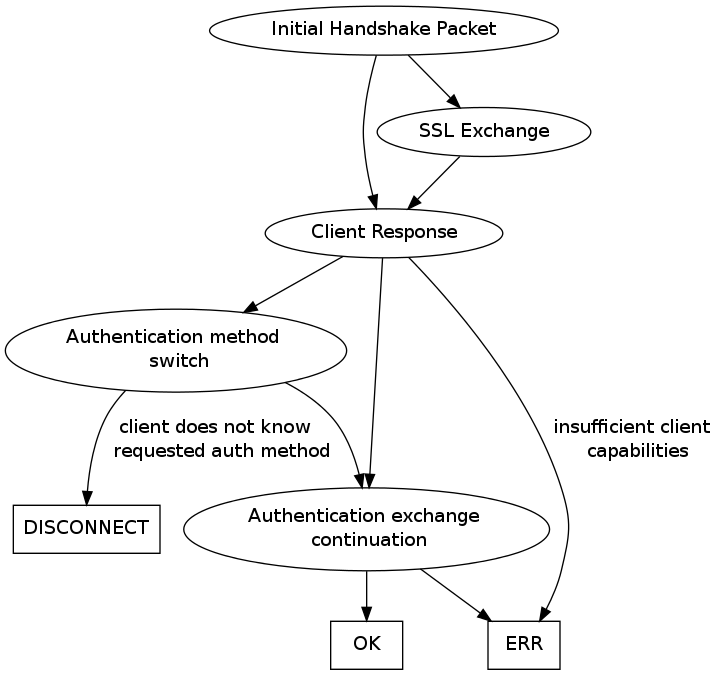
\includegraphics[width=5in]{002.png}
\end{center}

\subsection{握手}
握手开始于MySQL Server发送Protocol::Handshake,之后,客户端可以要求建立一个SSL通道(客户端发送Protocol::SSLRequest包),或直接发送Protocol::HandshakeResponse完成握手。

\subsubsection{普通握手方式}
MySQL Server发送Protocol::Handshake包,客户端响应Protocol::HandshakeResponse完成握手:
\begin{center}
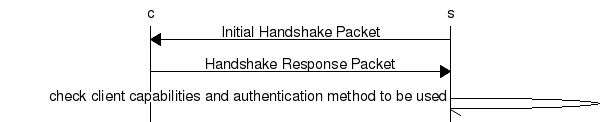
\includegraphics[width=6in]{003.png}
\end{center}

\subsubsection{SSL握手方式}
MySQL Server发送Protocol::Handshake、客户端响应Protocol::SSLRequest要求建立SSL通道、之后客户端和MySQL Server进行一系列标准的SSL交互建立SSL通道;通道建立之后,客户端发送Protocol::HandshakeResponse包完成握手:
\begin{center}
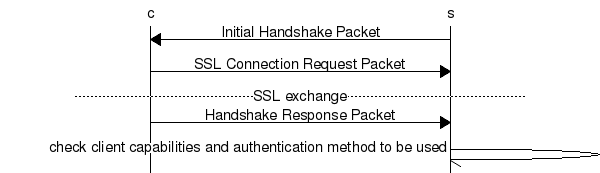
\includegraphics[width=6in]{004.png}
\end{center}

\subsubsection{能力交换}
为了兼容低版本的MySQL客户端,MySQL Server发送的Protocol::Handshake包中包含了:
\begin{itemize}
    \item MySQL Server的版本
    \item MySQL Server的能力,掩码表示。关于服务器的能力参考:\url{http://dev.mysql.com/doc/internals/en/capability-flags.html#packet-Protocol::CapabilityFlags}
\end{itemize}

客户端在Protocol::HandshakeResponse包中声明自己的能力。

\subsubsection{选择认证方法}
认证方法与用户的账号关联,存储在mysql.user表的plugin字段中。客户端发送的Protocol::HandshakeResponse包中包含了账号信息,MySQL Server根据账号信息查询mysql.user表获取认证方法。\\

实际使用中,为了减少一些网络交互,MySQL Server和客户端在握手阶段会采用一种乐观的方法选择认证方式:MySQL Server会在Protocol::Handshake带上缺省的认证方法、以及相关的数据;客户端在Protocol::HandshakeResponse包中会对是否选择默认的认证方法进行应答。\\

客户端可以不使用MySQL Server在Protocol::Handshake包中提议的认证方法,客户端将自己使用的认证方法加载到Protocol::HandshakeResponse包中发送给MySQL Server。当MySQL Server建议的认证方法和客户端使用的认证方法不同时,MySQL Server发送Protocol::AuthSwitchRequest包要求客户端使用包中表明的认证方法。\\

[TODO] MySQL旧有的密码认证方法、认证方法插件



\subsection{快速认证}
假设客户端以用户名U登录、使用的认证方法是M,当客户端和MySQL Server都使用方法M并在握手交互包中携带认证相关的数据时,就可以快速认证,认证的第一个阶段在握手就完成了。之后,客户端和MySQL Server根据认证方法的不同继续交换认证数据,直到认证成功或者失败。\\

一次快速认证成功的路径如下图所示:
\begin{center}
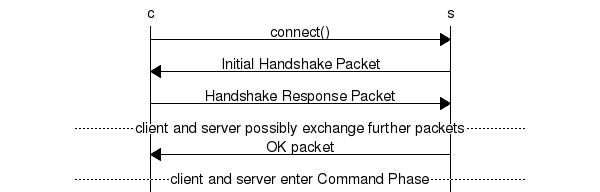
\includegraphics[width=6in]{005.png}
\end{center}

\begin{itemize}
    \item 客户端连接到MySQL Server
    \item MySQL发送Protocol::Handshake包,包中建议使用认证方法M
    \item 客户端发送Protocol::HandshakeResponse包,包中表明客户端也将使用方法M
    \item 客户端和MySQL Server根据M的要求持续发送认证数据,直到MySQL Server返回OK\_Packet
\end{itemize}

MySQL Server在阶段4发送的是Protocol::AuthMoreData包,包的前缀为0x01。\\

认证失败时,MySQL Server最后响应ERR\_Packet。

\subsection{认证方法不一致}
假设客户端以用户名U登录、使用的认证方法是M,当:
\begin{itemize}
    \item MySQL Server默认的认证方法不同于M
    \item 或客户端在Protocol::HandshakeResponse包中包含的认证方法不同于Protocol::Handshake包中建议的认证方法
\end{itemize}

客户端和MySQL Server需要重新协商选择正确的认证方法。MySQL Server发送Protocol::AuthMoreData包,包中包含了将要使用的认证方法、以及新方法产生的初始化认证数据。客户端应该使用新的认证方法并按照新方法的提示继续认证的过程。如果客户端不支持新的认证方法,则主动断开连接。

\subsubsection{更换认证方法}
步骤如下图所示:
\begin{center}
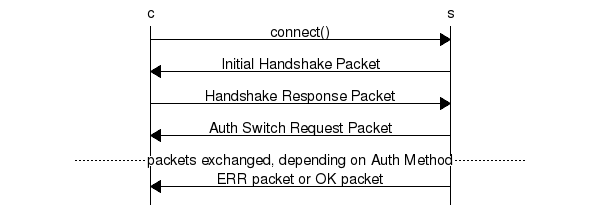
\includegraphics[width=6in]{006.png}
\end{center}

\subsubsection{客户端能力缺失}
当MySQL Server发现客户端的能力不足以完成认证过程时,发送ERR\_Packet并拒绝连接。以下情形会导致MySQL Server拒绝连接:
\begin{itemize}
    \item 一个不支持插件式认证(CLIENT\_PLUGIN\_AUTH没有设置)的客户端发起连接,提供的账号需要使用Secure Password Authentication或Old Password Authentication之外的认证方式
    \item 一个不支持安全认证(CLIENT\_SECURE\_CONNECTION没有设置)的客户端发起连接,提供的账号需要使用Old Password Authentication之外的认证方式
    \item MySQL Server缺省的认证方法不是Secure Password Authentication,并且客户端不支持插件式认证(CLIENT\_PLUGIN\_AUTH没有设置)
\end{itemize}

此时客户端和MySQL Server的交互过程如下:
\begin{center}
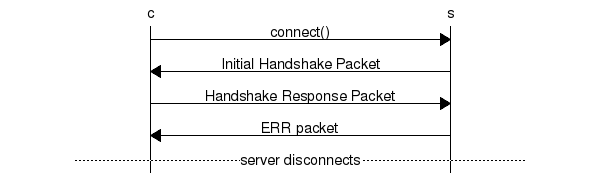
\includegraphics[width=6in]{007.png}
\end{center}

\subsubsection{客户端不支持新认证方法}
即使客户端支持外部的认证方法(CLIENT\_PLUGIN\_AUTH设置了),客户端也可能不支持新的认证方法,在这种情况下,客户端直接断开连接。\\

此时客户端和MySQL Server的交互过程如下:
\begin{center}
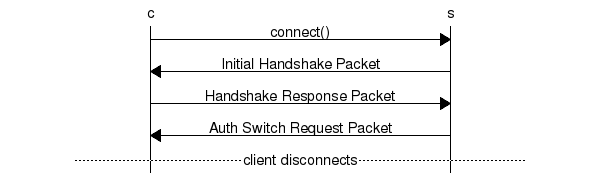
\includegraphics[width=6in]{008.png}
\end{center}

\subsubsection{不支持插件式认证方法的客户端}
[TODO]



\subsection{连接阶段消息包结构}
\subsubsection{Protocol::Handshake}
当客户端连接到MySQL Server时,MySQL Server向客户端发送Protocol::Handshake包,不同版本的MySQL Server、以及不同的配置导致Protocol::Handshake包的内容不同。\\

Protocol::Handshake包的格式如下:
\begin{center}
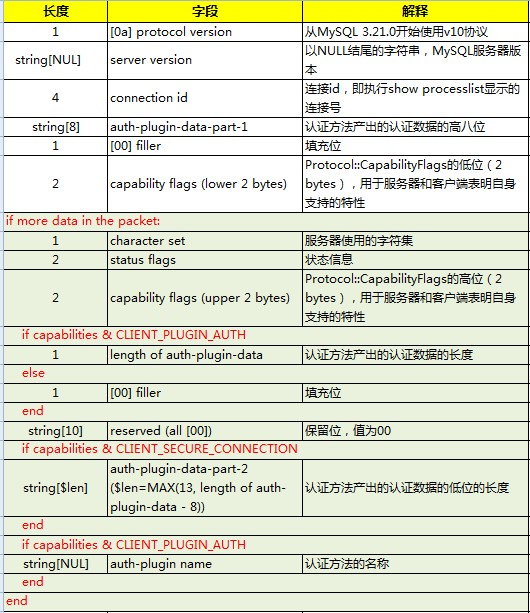
\includegraphics[width=5in]{009.jpg}
\end{center}

从MySQL 3.21.0开始使用v10协议。Handshake包中的capability类型为Protocol::Capability,具体含义参考\url{http://dev.mysql.com/doc/internals/en/capability-flags.html#packet-Protocol::CapabilityFlags}。\\

character set字段类型为Protocol::CharacterSet,具体含义参考\url{http://dev.mysql.com/doc/internals/en/character-set.html#packet-Protocol::CharacterSet}。\\

status flags字段类型为Protocol::StatusFlags,具体含义参考\url{http://dev.mysql.com/doc/internals/en/status-flags.html#packet-Protocol::StatusFlags}。\\

客户端接收到MySQL Server的Handshake包之后,发送HandshakeResponse包作为响应。

\subsubsection{Protocol::HandshakeResponse}
从MySQL 4.0开始使用HandshakeResponse41格式的协议包:
\begin{center}
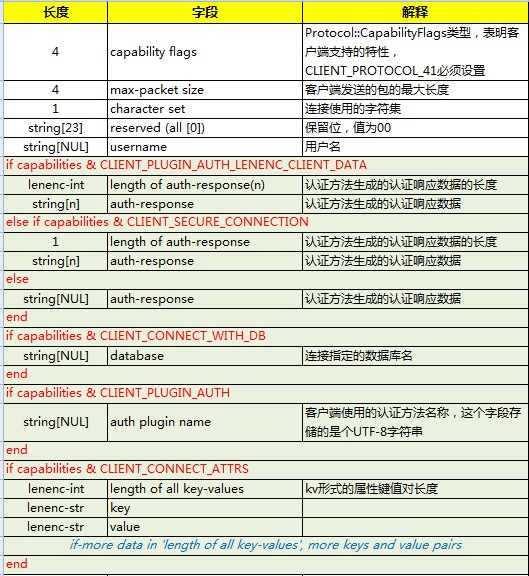
\includegraphics[width=5in]{010.jpg}
\end{center}

\newpage









\section{文本协议}
所谓文本协议,是指SQL语句中只包含文本,没有参数。当然了,这个查询SQL可以是select,也可以是update、delete、insert一类的。文本协议有很多,本文重点关注COM\_QUERY和相关协议。

\subsection{COM\_QUERY}
COM\_QUERY包的处理流程如下:
\begin{center}
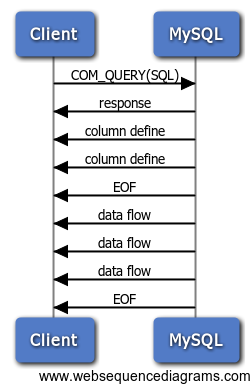
\includegraphics[width=3in]{011.png}
\end{center}

COM\_QUERY包格式如下:
\begin{center}
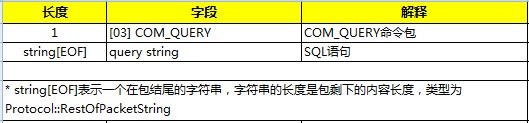
\includegraphics[width=5in]{012.jpg}
\end{center}

MySQL接收到COM\_QUERY之后进行处理,并把处理结果加载在COM\_QUERY\_RESPONSE类型的包中返回给客户端。

\subsection{COM\_QUERY\_RESPONSE}
COM\_QUERY\_RESPONSE实际是一个元数据包(meta packet),它可以是以下四种类型:
\begin{itemize}
    \item ERR\_Packet
    \item OK\_Packet
    \item Protocol::LOCAL\_INFILE\_Request
    \item ProtocolText::Resultset
\end{itemize}

COM\_QUERY\_RESPONSE的基本结构如下图所示:
\begin{center}
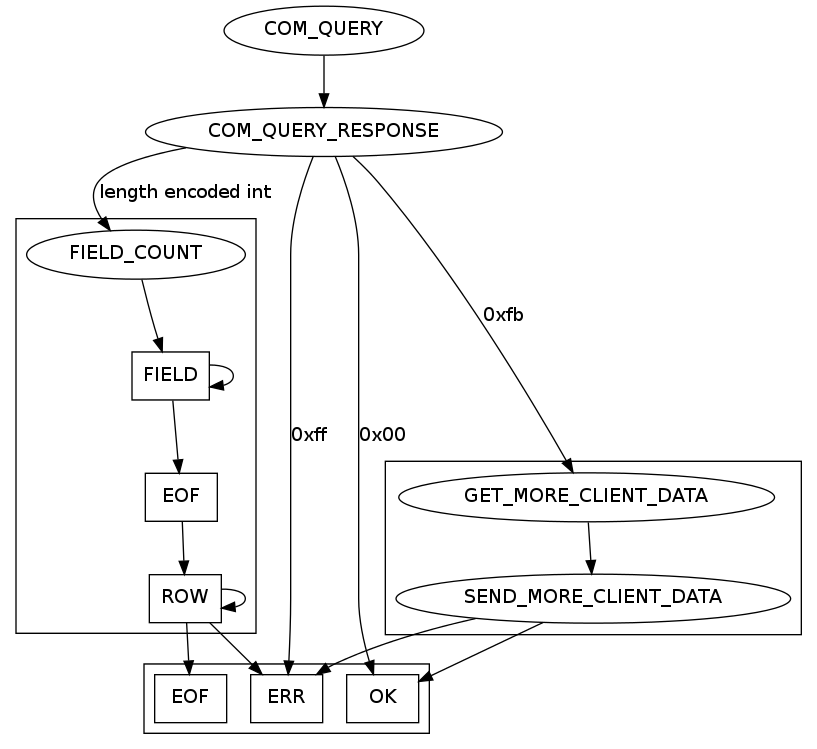
\includegraphics[width=5in]{013.png}
\end{center}

当COM\_QUERY\_RESPONSE的第一个byte是0x00,表示OK\_Packet;0xff表示一个ERR\_Packet;0xfb表示LOCAL\_INFILE\_Request包;否则,就是一个结果集(ResultSet)包。我们重点关注结果集包。\\

结果集由两个部分构成:
\begin{itemize}
    \item 列定义
    \item 行数据
\end{itemize}

一个语句的结果集可能由多个包构成。列定义部分由一个标示了列的个数的包开始、后续是包含列定义的内容的数据包,最后以一个OF\_Packet包结尾;数据部分由一系列包含行数据的包构成、以OF\_Packet包结尾。需要注意的是,如果MySQL Server能生成列定义部分、但是在生成行数据包的时候出错了,MySQL Server就会发送一个ERR\_Packet代替EOF\_Packet。\\

TextResult的基本结构如下:
\begin{center}
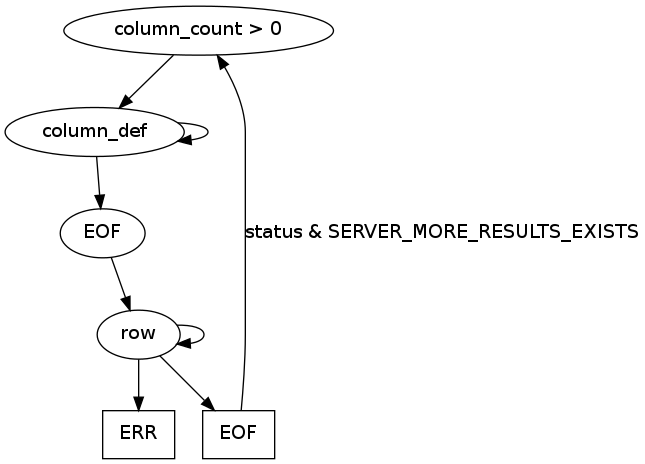
\includegraphics[width=5in]{014.png}
\end{center}

\subsubsection{列定义}
列定义包的类型为Protocol::ColumnDefinition。如果设置了CLIENT\_PROTOCOL\_41,则使用Protocol::ColumnDefinition41版本的格式;否则,使用Protocol::ColumnDefinition320。本文只关注41版本的格式。\\

Protocol::ColumnDefinition格式如下:
\begin{center}
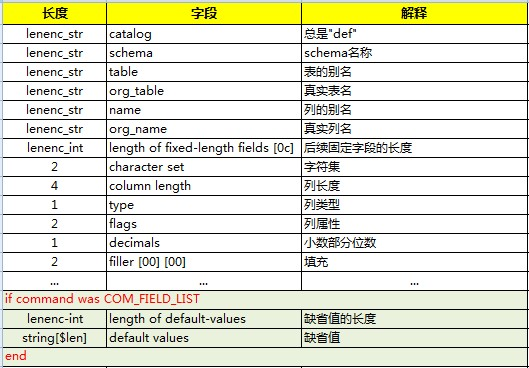
\includegraphics[width=5in]{015.jpg}
\end{center}

其中,列类型字段参考\url{http://dev.mysql.com/doc/internals/en/binary-protocol-value.html#packet-ProtocolBinary::MYSQL_TYPE_DECIMAL}。

\subsubsection{行数据}
行数据包类型为ProtocolText::ResultsetRow,除了NULL值由0xfb表示,其它的值都转换成Protocol::LengthEncodedString类型。

\newpage









\section{Binlog}
本章讨论MySQL Binlog的格式与应用。Binlog包含了在MySQL Server上执行的所有导致数据变化的操作。本章讨论的内容同样适用与MySQL Slave的Relay Log,Binlog和Relay Log的格式是完全相同的。

\subsection{什么是Binlog}
Binlog是MySQL Server实例在运行时产生的一系列文件(我们称之为Binary Log File),其中包含了所有对MySQL Server数据更改的信息。我们可以通过设置--log-bin选项启用Binlog。\\

Binlog最早出现在MySQL 3.23.14版本。最初的Binlog是基于语句的,也就是说Binlog记录了所有可能改变数据的SQL语句。之后,MySQL支持基于行的Binlog。基于行的Binlog不再记录SQL语句了,而是把SQL语句以“事件”的形式记录下来:事件以数据行为单位,描述了SQL语句执行前后数据的变化。\\

Binlog中还包含了一些元数据信息:
\begin{itemize}
    \item 所有确保Binlog记录的数据变化事件能够重现的MySQL Server状态信息
    \item 错误码
    \item 维护Binlog自身需要的元数据(比如rotate事件)
\end{itemize}

Binlog会跟踪记录MySQL Server运行时数据的变化,这些变化信息以“事件”的形式记录下来。换句话说,Binlog的“事件”可以重现MySQL Server数据的变化。\\

Binlog有两个重要的作用:
\begin{itemize}
    \item MySQL主备复制场景:首先在Replication Master Server上开启Binlog记录Master所有的数据变化;之后Master将Binlog发送到Replication Slave Server;Replication Slave Server先将Binlog转存为Relay Log(Relay Log与Binlog格式完全相同),之后将Relay Log中的事件重放,从而保证Replication Master和Slave的事件一致
    \item 一致的时间点恢复(PITR):通过mysqldump来做全备,然后通过Binlog记录之后所有的数据变更事件
\end{itemize}

通过下图,我们可以了解MySQL复制的基本原理、以及binlog在复制过程中所起的作用:
\begin{center}
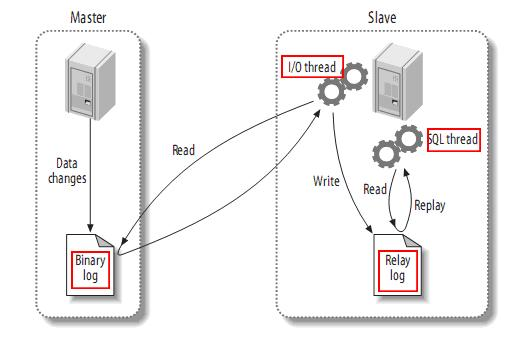
\includegraphics[width=5in]{019.png}
\end{center}

\subsubsection{Binlog格式}
MySQL Binlog日志有三种格式,分别为Statement、MiXED、以及ROW格式。传统意义上说,MySQL复制记录了产生变化的语句,称为基于语句的复制(Statement-based replication、SBR),此时Binlog记载了所有产生变化的SQL语句。基于语句的复制的缺点是无法保证所有的语句都正确复制,所以在MySQL 5.1版本中,MySQL提供了基于行的复制(Row-based replication、RBR),此时binlog以行为单位记录了数据库数据的变化。\\

行复制在某些情况下会产生大量的数据,比如当我们更新10000条记录的时候,基于行复制的binlog文件中就会记录这10000条记录变更的情况。在这种情况下,我们宁愿记录这条update语句,而不是10000条记录数据变化的情况。因此,MySQL又提供了一种Mixed格式的binlog文件。

\paragraph{基于语句的Binlog}
SBR每一条会修改数据的sql都会记录在Binlog中。\\

优点:不需要记录每一行的变化,减少了Binlog日志量,节约了IO,提高性能。(相比row能节约多少性能与日志量,这个取决于应用的SQL情况,正常同一条记录修改或者插入row格式所产生的日志量还小于Statement产生的日志量,但是考虑到如果带条件的update操作,以及整表删除,alter表等操作,ROW格式会产生大量日志,因此在考虑是否使用ROW格式日志时应该跟据应用的实际情况,其所产生的日志量会增加多少,以及带来的IO性能问题。)\\

缺点:由于记录的只是执行语句,为了这些语句能在slave上正确运行,因此还必须记录每条语句在执行的时候的一些相关信息,以保证所有语句能在slave得到和在master端执行时候相同的结果。另外mysql的复制,像一些特定函数功能,slave可与master上要保持一致会有很多相关问题(如sleep()函数、last\_insert\_id()、以及user defined functions(udf)会出现问题)。

使用以下函数的语句也无法被复制:
\begin{itemize}
    \item LOAD\_FILE()
    \item UUID()
    \item USER()
    \item FOUND\_ROWS()
    \item SYSDATE() (除非启动时启用了 --sysdate-is-now 选项)
    \item 在INSERT ...SELECT 会产生比RBR更多的行级锁
\end{itemize}

\paragraph{基于行的Binlog}
RBR不记录sql语句上下文相关信息,仅保存哪条记录被修改。\\

优点: Binlog中可以不记录执行的sql语句的上下文相关的信息,仅需要记录那一条记录被修改成什么了。所以rowlevel的日志内容会非常清楚的记录下每一行数据修改的细节。而且不会出现某些特定情况下的存储过程,或function,以及trigger的调用和触发无法被正确复制的问题。\\

缺点:所有的执行的语句当记录到日志中的时候,都将以每行记录的修改来记录,这样可能会产生大量的日志内容。比如一条update语句修改多条记录,则Binlog中每一条修改都会有记录,这样造成Binlog日志量会很大,特别是当执行alter table之类的语句的时候,由于表结构修改,每条记录都发生改变,那么该表每一条记录都会记录到日志中。

\paragraph{混合模式的binlog}
是以上两种level的混合使用,一般的语句修改使用statment格式保存Binlog,如一些函数;statement无法完成主从复制的操作,则采用row格式保存Binlog,MySQL会根据执行的每一条具体的sql语句来区分对待记录的日志形式,也就是在Statement和Row之间选择一种.新版本的MySQL中队row level模式也被做了优化,并不是所有的修改都会以row level来记录,像遇到表结构变更的时候就会以statement模式来记录。至于update或者delete等修改数据的语句,还是会记录所有行的变更。

\subsubsection{启用Binlog}
Mysql Binlog日志格式可以通过mysql的my.cnf文件的属性binlog\_format指定。比如:
\begin{spacing}{1.0}
\begin{lstlisting}
binlog_format = MIXED       //binlog日志格式
log_bin = ./mysql-bin.log   //binlog日志名
expire_logs_days = 7        //binlog过期清理时间
max_binlog_size = 100m      //binlog每个日志文件大小
\end{lstlisting}
\end{spacing}

按照上面的方法启用Binlog后,我们对数据库进行一系列操作:
\begin{spacing}{1.0}
\begin{lstlisting}
mysql> use test
Database changed

mysql> create table tbl(a int, b int);
iQuery OK, 0 rows affected (1.44 sec)

mysql> insert into tbl values(1,2);
Query OK, 1 row affected (0.13 sec)

mysql> flush logs;
Query OK, 0 rows affected (0.34 sec)
\end{lstlisting}
\end{spacing}

上述语句在test数据库实例中创建了表tbl、插入一条记录,然后让Binlog文件轮转。接下来可以观察到以下的Binlog事件:
\begin{spacing}{1.0}
\begin{lstlisting}
mysql> show binlog events in 'mysql-bin.000003'\G
*************************** 1. row ***************************
   Log_name: mysql-bin.000003
        Pos: 4
 Event_type: Format_desc
  Server_id: 1
End_log_pos: 120
       Info: Server ver: 5.6.17-65.0-log, Binlog ver: 4
*************************** 2. row ***************************
   Log_name: mysql-bin.000003
        Pos: 120
 Event_type: Query
  Server_id: 1
End_log_pos: 224
       Info: use `test`; create table tbl(a int, b int)
*************************** 3. row ***************************
   Log_name: mysql-bin.000003
        Pos: 224
 Event_type: Query
  Server_id: 1
End_log_pos: 303
       Info: BEGIN
*************************** 4. row ***************************
   Log_name: mysql-bin.000003
        Pos: 303
 Event_type: Query
  Server_id: 1
End_log_pos: 404
       Info: use `test`; insert into tbl values(1,2)
*************************** 5. row ***************************
   Log_name: mysql-bin.000003
        Pos: 404
 Event_type: Xid
  Server_id: 1
End_log_pos: 435
       Info: COMMIT /* xid=46 */
*************************** 6. row ***************************
   Log_name: mysql-bin.000003
        Pos: 435
 Event_type: Rotate
  Server_id: 1
End_log_pos: 482
       Info: mysql-bin.000004;pos=4
6 rows in set (0.00 sec)
\end{lstlisting}
\end{spacing}

这个Binlog文件中包含了一个格式描述事件、三个查询事件、一个Xid事件和一个日志轮转事件。后续章节会对每个事件进行详细描述,这里只简单看一下每个事件包含的字段:
\begin{itemize}
    \item Log\_name:这个事件所在的Binary Log File名称.这里是在mysql-bin.000005
    \item Pos:这个事件在当前Binary Log File中的位置
    \item Event\_type:这个事件的类型,类型是有很多,用来记录数据库的操作
    \item Server\_id:这个事件是在哪个server上发生的。注意在replication中,这个server id记录的是master端的server id
    \item End\_log\_pos:下一个事件的位置。因此当前这个event的长度是End\_log\_pos-Pos
    \item Info:直观可读的关于事件的信息
\end{itemize}

\subsubsection{Binlog结构与内容小结}
通过上面的描述,我们对Binlog的结构与内容有了大致的认识,这里对上面的内容做一个简单的总结:
\begin{itemize}
    \item Binlog是由一组Binary Log File和Index File构成
    \item 每个Binary Log File由4 byte的magic number开头,后续是一系列事件,描述了数据的变更状况:
    \begin{itemize}
        \item magic number值为0xfe 0x62 0x69 0x6e(即0xfe 'b''i''n')
        \item 每个事件都包括了事件头和数据部分:
        \begin{itemize}
            \item 事件头包含了事件类型、产生时间、服务器标识等等
            \item 数据部分与事件类型有关
        \end{itemize}
    \end{itemize}
    \item Binary Log File的第一个事件是描述事件,表明了这个Binary Log File文件的版本(即描述事件使用的格式信息)
    \item Binary Log File的最后一个事件是日志轮转事件,包含了下一个Binary Log File的文件名
\end{itemize}

Binary Log File的默认命名规则为"HOSTNAME-bin.NNNNNN",Index文件的默认命名规则为“HOSTNAME-bin.index”,其中NNNNNN以1为单位递增。\\

Relay Log File的命名规则类似,只是在将前缀中的bin改为relay:"HOSTNAME-relay.NNNNNN"、"HOSTNAME-relay.index"。



\subsection{Binlog事件}
\subsubsection{事件定义}
Binlog事件在log\_event.h文件中定义,代码如下:
\begin{spacing}{1.0}
\begin{lstlisting}
enum Log_event_type { 
  UNKNOWN_EVENT= 0, 
  START_EVENT_V3= 1, 
  QUERY_EVENT= 2, 
  STOP_EVENT= 3, 
  ROTATE_EVENT= 4, 
  INTVAR_EVENT= 5, 
  LOAD_EVENT= 6, 
  SLAVE_EVENT= 7, 
  CREATE_FILE_EVENT= 8, 
  APPEND_BLOCK_EVENT= 9, 
  EXEC_LOAD_EVENT= 10, 
  DELETE_FILE_EVENT= 11, 
  NEW_LOAD_EVENT= 12, 
  RAND_EVENT= 13, 
  USER_VAR_EVENT= 14, 
  FORMAT_DESCRIPTION_EVENT= 15, 
  XID_EVENT= 16, 
  BEGIN_LOAD_QUERY_EVENT= 17, 
  EXECUTE_LOAD_QUERY_EVENT= 18, 
  TABLE_MAP_EVENT = 19, 
  PRE_GA_WRITE_ROWS_EVENT = 20, 
  PRE_GA_UPDATE_ROWS_EVENT = 21, 
  PRE_GA_DELETE_ROWS_EVENT = 22, 
  WRITE_ROWS_EVENT = 23, 
  UPDATE_ROWS_EVENT = 24, 
  DELETE_ROWS_EVENT = 25, 
  INCIDENT_EVENT= 26, 
  HEARTBEAT_LOG_EVENT= 27, 
  ENUM_END_EVENT 
  /* end marker */ 
};
\end{lstlisting}
\end{spacing}

事件按用途分类如下:
\begin{itemize}
    \item Binlog管理:
        \begin{itemize}
            \item START\_EVENT\_V3
            \item FORMAT\_DESCRIPTION\_EVENT
            \item STOP\_EVENT
            \item ROTATE\_EVENT
            \item SLAVE\_EVENT
            \item INCIDENT\_EVENT
            \item HEARTBEAT\_EVENT
        \end{itemize}
    \item SBR相关事件:
        \begin{itemize}
            \item QUERY\_EVENT
            \item INTVAR\_EVENT
            \item RAND\_EVENT
            \item USER\_VAR\_EVENT
            \item XID\_EVENT
        \end{itemize}
    \item RBR相关事件:
        \begin{itemize}
            \item TABLE\_MAP\_EVENT
            \item DELETE\_ROWS\_EVENTv0
            \item UPDATE\_ROWS\_EVENTv0
            \item WRITE\_ROWS\_EVENTv0
            \item DELETE\_ROWS\_EVENTv1
            \item UPDATE\_ROWS\_EVENTv1
            \item WRITE\_ROWS\_EVENTv1
            \item DELETE\_ROWS\_EVENTv2
            \item UPDATE\_ROWS\_EVENTv2
            \item WRITE\_ROWS\_EVENTv2
        \end{itemize}
    \item Load INFILE相关事件:
        \begin{itemize}
            \item LOAD\_EVENT
            \item CREATE\_FILE\_EVENT
            \item APPEND\_BLOCK\_EVENT
            \item EXEC\_LOAD\_EVENT
            \item DELETE\_FILE\_EVENT
            \item NEW\_LOAD\_EVENT
            \item BEGIN\_LOAD\_QUERY\_EVENT
            \item EXECUTE\_LOAD\_QUERY\_EVENT
        \end{itemize}
\end{itemize}

\subsubsection{事件描述}
事件描述(这里只描述了MySQL 5.0之后还在使用的事件、以及RBL格式的事件):
\begin{itemize}
    \item UNKNOWN\_EVENT:如果从Binary Log File中读出的事件类型不在类型定义范围内,那么这个事件就被认为是一个UNKNOWN\_EVENT
    \item QUERY\_EVENT:执行一个引起数据变化的DML语句
    \item STOP\_EVENT:mysqld进程停止
    \item ROTATE\_EVENT:mysqld切换一个新的Binary Log File。这个事件发生有两种情况,一是用户执行了Flush Logs命令,二是一个Binary Log File大小超过了max\_binlog\_size
    \item FORMAT\_DESCRIPTION\_EVENT:每个Binary Log File第一个事件,包含了服务器ID、Binlog版本号等
    \item BEGIN\_LOAD\_QUERY\_EVENT:用于LOAD DATA INFILE语句
    \item EXECUTE\_LOAD\_QUERY\_EVENT:用于LOAD DATA INFILE语句
    \item TABLE\_MAP\_EVENT:用于RBL格式的日志,记录了下一条事件所对应的表信息,在其中存储了数据库名和表名。使用这个事件的目的是为了在Replication Master和Slave表的定义不同时复制数据
    \item WRITE\_ROWS\_EVENT:记录了对单表的insert操作
    \item UPDATE\_ROWS\_EVENT:记录了对单表的update操作
    \item DELETE\_ROWS\_EVENT:记录了对单表的delete操作
    \item INCIDENT\_EVENT:Used to log an out of the ordinary event that occurred on the master. It notifies the slave that something happened on the master that might cause data to be in an inconsistent state.
    \item HEARTBEAT\_LOG\_EVENT:Master和Slave之间的心跳事件,注意:这个事件不会记录在Binary Log File中
\end{itemize}

\subsubsection{事件结构}
所有的Binlog事件都遵循相同的格式:固定的事件头和变长的事件数据 ,如下图所示:
\begin{center}
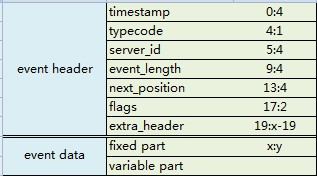
\includegraphics[width=4in]{020.jpg}
\end{center}

其中,flags字段含义参考\url{http://dev.mysql.com/doc/internals/en/event-flags.html}。

\subsubsection{FORMAT\_DESCRIPTION\_EVENT}
FORMAT\_DESCRIPTION\_EVENT事件是Binary Log File中的第一个事件,记录了Binlog的版本、MySQL Server的版本号、其它事件头的长度(总是19)、事件的附加头长度。FORMAT\_DESCRIPTION\_EVENT的格式如下图所示:
\begin{center}
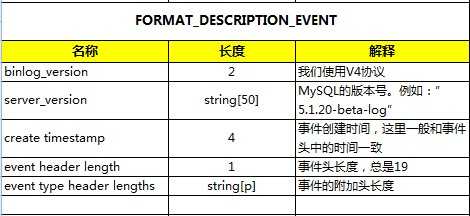
\includegraphics[width=5in]{021.jpg}
\end{center}

[TODO]:附加头长度的计算方法

\subsubsection{ROTATE\_EVENT}
mysqld切换一个新的Binary Log File时会产生ROTATE\_EVENT,换句话说,ROTATE\_EVENT总在Binary Log File的尾部。ROTATE\_EVENT事件发生有两种情况,一是用户执行了Flush Logs命令,二是一个Binary Log File大小超过了max\_binlog\_size。\\

ROTATE\_EVENT事件的格式如下:
\begin{center}
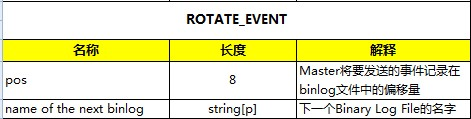
\includegraphics[width=5in]{022.jpg}
\end{center}

\subsubsection{TABLE\_MAP\_EVENT}
TABLE\_MAP\_EVENT记录了下一条事件所对应的表信息,格式如下所示:
\begin{center}
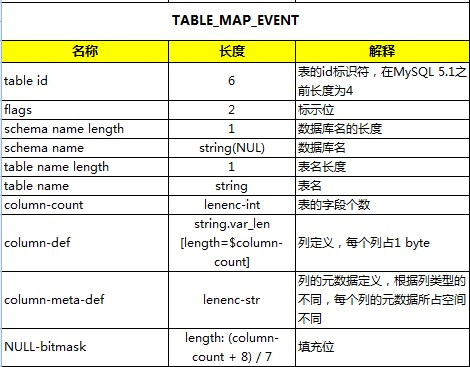
\includegraphics[width=5in]{023.jpg}
\end{center}

TABLE\_MAP\_EVENT以事务为单位组织,每个事务的第一个事件必须是TABLE\_MAP\_EVENT,之后是一系列的WRITE\_ROWS\_EVENT、UPDATE\_ROWS\_EVENT或DELETE\_ROWS\_EVENT,如下图所示:
\begin{center}
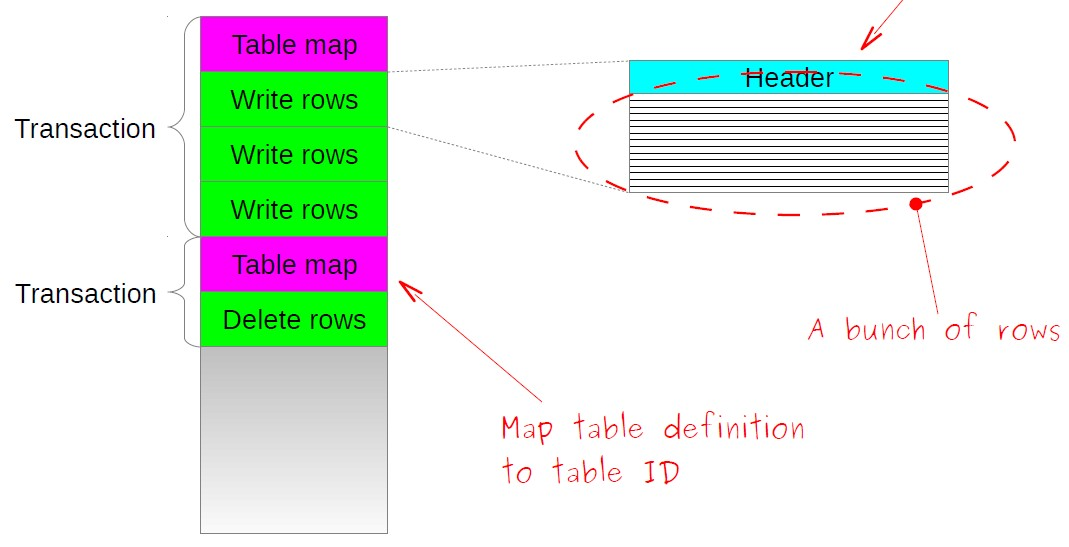
\includegraphics[width=5in]{024.jpg}
\end{center}

\subsubsection{ROWS\_EVENT}
ROWS\_EVENT是WRITE\_ROWS\_EVENT、UPDATE\_ROWS\_EVENT和DELETE\_ROWS\_EVENT的统称,分别记录了insert、update和delete语句对应的Binlog事件。ROWS\_EVENT经历了v0、v1和v2共三个版本,其中v0版在MySQL 5.1.15之后就不在使用了,v1版在5.6之后不再使用,我们这里介绍v2版本的ROWS\_EVENT事件。\\

WRITE\_ROWS\_EVENT、UPDATE\_ROWS\_EVENT和DELETE\_ROWS\_EVENT的格式类似,如下图所示:
\begin{center}
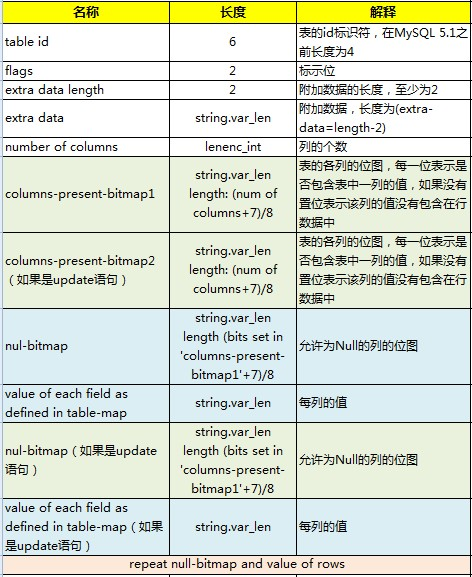
\includegraphics[width=5in]{025.jpg}
\end{center}

需要注意两个字段的用途:
\begin{itemize}
    \item columns-present-bitmap:每个bit表示一个列,如果bit置位了,表示该列的数据包含在后续的“行数据”部分。[TODO:我还没想到那种场景下会有没置位的情况]
    \item nul-bitmap:每个bit表示列的值是否为Null
\end{itemize}



\subsection{监听流程}
客户端向MySQL Server发送COM\_BINLOG\_DUMP后等待MySQL将Binlog事件回送。COM\_BINLOG\_DUMP的格式如下:
\begin{center}
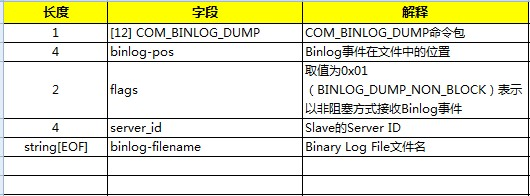
\includegraphics[width=5in]{026.jpg}
\end{center}

\newpage











\section{代码实现(基于Golang)}
基于Golang的MySQL Driver实现(GoMySQL),简单起见,并没有遵守database/sql/driver接口协议。

\subsection{模块布局}
GoMySQL包含了以下主要模块:
\begin{center}
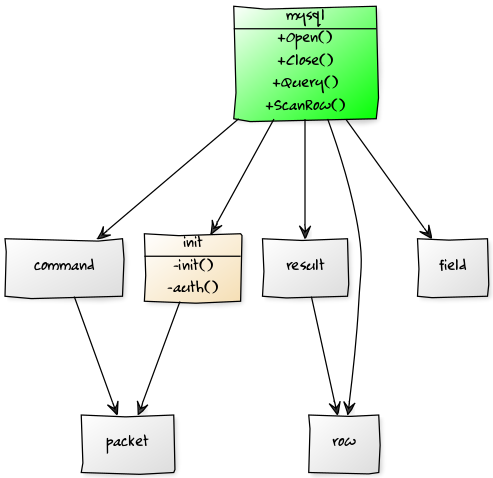
\includegraphics[width=5in]{016.png}
\end{center}

其中:
\begin{itemize}
    \item mysql模块:对外提供接口,包括数据库连接、关闭、SQL执行、结果集遍历以及binlog事件监听等等
    \item init模块:处理客户端与MySQL Server的握手和认证信息
    \item command模块:处理文本模式的协议
    \item result模块:结果集
    \item row模块:行数据
    \item field模块:列定义
    \item packet模块:网络层包读写相关操作
\end{itemize}

GoMySQL的功能主要包括:
\begin{itemize}
    \item 上下文管理
    \item Packet读写
    \item 编解码
    \item 数据库连接
    \item 查询语句处理
    \item 结果集处理
    \item binlog时间监听
\end{itemize}

后续我们将以功能为单元依次展开讨论。



\subsection{上下文管理}
上下文管理功能包含在mysql模块的两个结构体中,定义如下:
\begin{spacing}{1.0}
\begin{lstlisting}
// infomation from handshake packet
type serverInfo struct {
    protocol_version    byte  
    server_version      []byte 
    connection_id       uint32 
    scramble            [20]byte  
    capability          uint16      
    lang                byte     
}

// MySQL connection handler
type MySQL struct {
    protocol        string      // Network protocol
    address         string      // Server address
    user            string      // MySQL username
    passwd          string      // MySQL password
    dbname          string      // Database name

    socket          net.Conn    // MySQL connection
    rd              *bufio.Reader
    wr              *bufio.Writer

    info            serverInfo  // MySQL server information
    seq             byte        // MySQL sequence number
    status          uint16      // Current status of MySQL server connection
    max_pkt_size    int         // Maximum packet size that client can accept from server
    timeout         time.Duration // Timeout for connect
}
\end{lstlisting}
\end{spacing}

serverInfo结构体用于保存MySQL Server发送的Handshake消息包的内容,包括协议版本号、Server版本信息、连接ID(即执行show processlist语句显示的ID)、Server缺省认证方法产生的认证数据、Server支持的特性、以及Server使用的字符集信息。\\

MySQL结构体保存了一个客户端和MySQL Server连接的上下文信息,包括了如下信息:
\begin{itemize}
    \item 连接使用的协议族
    \item Server地址
    \item 连接使用的用户名和密码
    \item 连接的数据库实例名
    \item 连接底层的socket句柄以及读写缓冲区
    \item Handshake携带的Server信息
    \item 当前包的序列号
    \item 连接状态
    \item 包允许的最大尺寸
    \item 连接超时时间
\end{itemize}



\subsection{Packet读写}
客户端和MySQL Server通过数据包(packet)进行交互,packet的基本结构如下:
\begin{center}
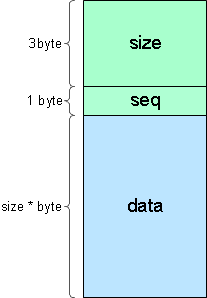
\includegraphics[width=2in]{017.png}
\end{center}

Packet读写功能由packet模块处理。packet模块包含了pktReader和pktWriter两个结构体分别用于实现packet的读和写。

\subsubsection{pktReader}
pktReader的结构如下:
\begin{spacing}{1.0}
\begin{lstlisting}
type pktReader struct {
  rd     *bufio.Reader
  seq    *byte
  remain int
  last   bool
  buf    [8]byte
  ibuf   [3]byte
}
\end{lstlisting}
\end{spacing}

其中包含了:
\begin{itemize}
    \item rd:底层socket读缓冲
    \item seq:序列号,从0开始
    \item remain:数据包的长度(不包括包头4个byte)
    \item last:当包大于16M时会分包,last用于表示是否是最后一个包
    \item buf:
    \item ibuf:3个byte的数组,用于读取包头的size字段
\end{itemize}

pktReader.newPktReader()构造一个pktReader对象:
\begin{spacing}{1.0}
\begin{lstlisting}
func (my *MySQL) newPktReader() *pktReader {
  return &pktReader{rd: my.rd, seq: &my.seq}
}
\end{lstlisting}
\end{spacing}

pktReader.readHeader()读取包头的内容(首先读取3 byte的包长度,然后读取seq,最后判断是否是最后一个包):
\begin{spacing}{1.0}
\begin{lstlisting}
func (pr *pktReader) readHeader() {
  buf := pr.ibuf[:]
  for {
    n, err := pr.rd.Read(buf)
    if err != nil { panic(err) }
    buf = buf[n:]
    if len(buf) == 0 { break }
  }
  pr.remain = int(DecodeU24(pr.ibuf[:]))
  seq, err := pr.rd.ReadByte()
  if err != nil { panic(err) }

  // Chceck sequence number
  if *pr.seq != seq { panic(ErrSeq) }
  *pr.seq++

  // Last packet?
  pr.last = (pr.remain != 0xffffff)
}
\end{lstlisting}
\end{spacing}

pktReader.readFull(buf []byte)方法读取buf长度的内容:
\begin{spacing}{1.0}
\begin{lstlisting}
func (pr *pktReader) readFull(buf []byte) {
  for len(buf) > 0 {
    if pr.remain == 0 {
      if pr.last { panic(io.EOF) }
      pr.readHeader()
    }
    n := len(buf)
    if n > pr.remain { n = pr.remain }
    n, err := pr.rd.Read(buf[:n])
    pr.remain -= n
    if err != nil { panic(err) }
    buf = buf[n:]
  }
  return
}
\end{lstlisting}
\end{spacing}

pktReader.readAll(buf []byte)方法读取包数据部分的内容长度的内容:
\begin{spacing}{1.0}
\begin{lstlisting}
func (pr *pktReader) readAll() (buf []byte) {
  m := 0
  for {
    if pr.remain == 0 {
      if pr.last { break }
      pr.readHeader()
    }
    new_buf := make([]byte, m+pr.remain)
    copy(new_buf, buf)
    buf = new_buf
    n, err := pr.rd.Read(buf[m:])
    pr.remain -= n
    m += n
    if err != nil { panic(err) }
  }
  return
}
\end{lstlisting}
\end{spacing}

其它的方法包括:
\begin{itemize}
    \item readByte():读取一个byte
    \item skipAll():读取但不缓冲包中剩余的数据
    \item skipN(n int):读取但不缓冲包中N byte的数据
    \item unreadByte():回退一个byte。只有刚读取并且没有被消费掉的内容才能回退
\end{itemize}

\subsubsection{pktWriter}
pkt Writer的结构如下:
\begin{spacing}{1.0}
\begin{lstlisting}
type pktWriter struct {
  wr       *bufio.Writer
  seq      *byte
  remain   int
  to_write int
  last     bool
  buf      [23]byte
  ibuf     [3]byte
}
\end{lstlisting}
\end{spacing}

其中包含了:
\begin{itemize}
    \item wr:底层socket写缓冲
    \item seq:序列号,从0开始
    \item remain:数据包的长度(不包括包头4个byte)
    \item to\_write:将要写入的数据长度
    \item last:当包大于16M时会分包,last用于表示是否是最后一个包
    \item buf:
    \item ibuf:3个byte的数组,用于写入包头的size字段
\end{itemize}

pktWriter.newPktWriter()初始化一个pktWriter对象:
\begin{spacing}{1.0}
\begin{lstlisting}
func (my *MySQL) newPktWriter(to_write int) *pktWriter {
  return &pktWriter{wr: my.wr, seq: &my.seq, to_write: to_write}
}
\end{lstlisting}
\end{spacing}

pktReader.writeHeader()组装包头的内容并写入发送缓冲:
\begin{spacing}{1.0}
\begin{lstlisting}
func (pw *pktWriter) writeHeader(l int) {
  buf := pw.ibuf[:]
  EncodeU24(buf, uint32(l))
  if _, err := pw.wr.Write(buf); err != nil {
    panic(err)
  }
  if err := pw.wr.WriteByte(*pw.seq); err != nil {
    panic(err)
  }
  // Update sequence number
  *pw.seq++
}
\end{lstlisting}
\end{spacing}

pktReader.write(buf []byte)将buf内容写入发送缓冲区:
\begin{spacing}{1.0}
\begin{lstlisting}
func (pw *pktWriter) write(buf []byte) {
  if len(buf) == 0 {
    return
  }
  var nn int
  for len(buf) != 0 {
    if pw.remain == 0 {
      if pw.to_write == 0 { panic("too many data for write as packet") }
      if pw.to_write >= 0xffffff {
        pw.remain = 0xffffff
      } else {
        pw.remain = pw.to_write
        pw.last = true
      }
      pw.to_write -= pw.remain
      pw.writeHeader(pw.remain)
    }
    
    nn = len(buf)
    if nn > pw.remain { nn = pw.remain }

    var err error
    nn, err = pw.wr.Write(buf[0:nn])
    pw.remain -= nn
    if err != nil { panic(err) }
    buf = buf[nn:]
  }
  if pw.remain+pw.to_write == 0 {
    if !pw.last { pw.writeHeader(0) }
    if err := pw.wr.Flush(); err != nil { panic(err) }
  }
  return
}
\end{lstlisting}
\end{spacing}

需要主要的是,当写入的内容长度大于0xffffff时,必须分多个packet写入。



\subsection{编解码}
codecs模块提供编解码功能,包含了一系列不同类型的编解码函数以及对应的网络发送接收缓冲的读写操作:
\begin{itemize}
    \item 16、24、32、64位无符号整数
    \item 变长整数类型(即Protocol::LengthEncodedInteger)
    \item 变长的字符串(即Protocol::LengthEncodedString)
    \item 以0结尾的字符串
    \item 时间相关类型
\end{itemize}

我们以16位整数为例分析编解码以及接收发送的相关实现:
\begin{spacing}{1.0}
\begin{lstlisting}
func DecodeU16(buf []byte) uint16 {
  return uint16(buf[1])<<8 | uint16(buf[0])
}

func (pr *pktReader) readU16() uint16 {
  buf := pr.buf[:2]
  pr.readFull(buf)
  return DecodeU16(buf)
}

func EncodeU16(buf []byte, val uint16) {
  buf[0] = byte(val)
  buf[1] = byte(val >> 8)
}

func (pw *pktWriter) writeU16(val uint16) {
  buf := pw.buf[:2]
  EncodeU16(buf, val)
  pw.write(buf)
}
\end{lstlisting}
\end{spacing}

Protocol::LengthEncodedInteger类型的发送和接收函数实现如下(Protocol::LengthEncodedInteger参考本文[基本类型]一节):
\begin{spacing}{1.0}
\begin{lstlisting}
func (pr *pktReader) readNullLCB() (lcb uint64, null bool) {
  bb := pr.readByte()
  switch bb {
  case 251:
    null = true
  case 252:
    lcb = uint64(pr.readU16())
  case 253:
    lcb = uint64(pr.readU24())
  case 254:
    lcb = pr.readU64()
  default:
    lcb = uint64(bb)
  }
  return
}

func (pw *pktWriter) writeLCB(val uint64) {
  switch {
  case val <= 250:
    pw.writeByte(byte(val))
  case val <= 0xffff:
    pw.writeByte(252)
    pw.writeU16(uint16(val))
  case val <= 0xffffff:
    pw.writeByte(253)
    pw.writeU24(uint32(val))
  default:
    pw.writeByte(254)
    pw.writeU64(val)
  }
}
\end{lstlisting}
\end{spacing}

Protocol::LengthEncodedString类型的发送接收函数实现如下(Protocol::LengthEncodedString参考本文[基本类型]一节):
\begin{spacing}{1.0}
\begin{lstlisting}
func (pr *pktReader) readNullBin() (buf []byte, null bool) {
  var l uint64
  l, null = pr.readNullLCB()
  if null {
    return
  }
  buf = make([]byte, l)
  pr.readFull(buf)
  return
}

func (pw *pktWriter) writeBin(buf []byte) {
  pw.writeLCB(uint64(len(buf)))
  pw.write(buf)
}

func (pw *pktWriter) writeLC(v interface{}) {
  switch val := v.(type) {
  case []byte:
    pw.writeBin(val)
  case *[]byte:
    pw.writeBin(*val)
  case string:
    pw.writeBin([]byte(val))
  case *string:
    pw.writeBin([]byte(*val))
  default:
    panic("Unknown data type for write as length coded string")
  }
}
\end{lstlisting}
\end{spacing}

以0结尾的字符串接收发送函数实现如下:
\begin{spacing}{1.0}
\begin{lstlisting}
func (pr *pktReader) readNTB() (buf []byte) {
  for {
    ch := pr.readByte()
    if ch == 0 {
      break
    }
    buf = append(buf, ch)
  }
  return
}

func (pw *pktWriter) writeNTB(buf []byte) {
  pw.write(buf)
  pw.writeByte(0)
}
\end{lstlisting}
\end{spacing}



\subsection{数据库连接}
mysql模块的Open()方法用于建立数据库连接,基本实现如下:
\begin{spacing}{1.0}
\begin{lstlisting}
func Open(protocol, address, user, passwd, dbname string) (*MySQL, error) {
    my := &MySQL {
        protocol:      protocol,
        address:       address,
        user:          user,
        passwd:        passwd,
        dbname:        dbname,
        max_pkt_size:  16*1024*1024 - 1,
        timeout:       2 * time.Minute,
        fullFieldInfo: true,
    };

    var err error;
    my.socket, err = net.Dial(protocol, address);
    if err != nil { return nil, err; }

    my.rd = bufio.NewReader(my.socket);
    my.wr = bufio.NewWriter(my.socket);

    // Initialisation
    my.init()
    my.auth()

    res := my.getResult(nil, nil)
    if res == nil {
        // Try old password
        my.oldPasswd()
        res = my.getResult(nil, nil)
        if res == nil { return nil, ErrAuthentication }
    }
    return my, nil;
}
\end{lstlisting}
\end{spacing}
Open()方法首先将连接使用的用户名、密码、服务器地址以及要连接的数据库实例名保存在上下文中,之后建立Socket连接、管理Socket读写缓冲区。底层Socket连接成功之后,就可以接收并Server端发送的Handshake包,实现握手和认证过程。

\subsubsection{握手阶段}
客户端与MySQL Server建立连接之后,Server会发送一个Handshake包。init模块中的init()方法用于处理Handshake包:
\begin{spacing}{1.0}
\begin{lstlisting}
func (my *MySQL) init() {
    my.seq = 0; // Reset sequence number, mainly for reconnect

    pr := my.newPktReader();
    my.info.protocol_version = pr.readByte();
    my.info.server_version = pr.readNTB();
    my.info.connection_id = pr.readU32();
    pr.readFull(my.info.scramble[0:8]);
    pr.skipN(1);
    my.info.capability = pr.readU16();
    my.info.lang = pr.readByte();
    my.status = pr.readU16();
    pr.skipN(13);
    if my.info.capability&_CLIENT_PROTOCOL_41 != 0 {
        pr.readFull(my.info.scramble[8:]);
    }
    pr.skipAll(); // Skip other information
    if my.info.capability&_CLIENT_PROTOCOL_41 == 0 {
        panic(ErrOldProtocol)
    }
}
\end{lstlisting}
\end{spacing}

\subsubsection{认证阶段}
客户端发送HandshakeResponse包,携带认证相关信息完成认证过程,具体实现如下:
\begin{spacing}{1.0}
\begin{lstlisting}
func (my *MySQL) auth() {
    my.debug("[%2d <-] Authentication packet", my.seq);
    flags := uint32(
        _CLIENT_PROTOCOL_41 |
            _CLIENT_LONG_PASSWORD |
            _CLIENT_LONG_FLAG |
            _CLIENT_TRANSACTIONS |
            _CLIENT_SECURE_CONN |
            _CLIENT_LOCAL_FILES |
            _CLIENT_MULTI_STATEMENTS |
            _CLIENT_MULTI_RESULTS)
    // Reset flags not supported by server
    flags &= uint32(my.info.capability) | 0xffff0000
    scrPasswd := encryptedPasswd()(my.passwd, my.info.scramble[:])
    pay_len := 4 + 4 + 1 + 23 + len(my.user) + 1 + 1 + len(scrPasswd)
    if len(my.dbname) > 0 {
        pay_len += len(my.dbname) + 1
        flags |= _CLIENT_CONNECT_WITH_DB
    }
    pw := my.newPktWriter(pay_len)
    pw.writeU32(flags)
    pw.writeU32(uint32(my.max_pkt_size))
    pw.writeByte(my.info.lang)   // Charset number
    pw.writeZeros(23)            // Filler
    pw.writeNTB([]byte(my.user)) // Username
    pw.writeBin(scrPasswd)       // Encrypted password
    if len(my.dbname) > 0 {
        pw.writeNTB([]byte(my.dbname))
    }
    if len(my.dbname) > 0 {
        pay_len += len(my.dbname) + 1
        flags |= _CLIENT_CONNECT_WITH_DB
    }
    return
}
\end{lstlisting}
\end{spacing}

认证阶段比较复杂的是密码身份认证,我们已经将身份认证的步骤封装在encryptedPasswd(),这里简单介绍一下MySQL身份认证的方法。\\

MySQL的身份认证协议是一种CHAP协议,即,挑战应答:
\begin{center}
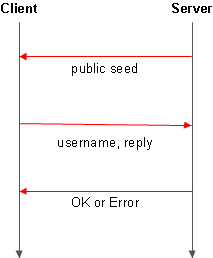
\includegraphics[width=2in]{018.png}
\end{center}

首先,我们知道,用户密码是保存在mysql.user这个表的password列,并且是以hash值的形式加密保存的。\\

整个验证过程如下,当客户端请求连接时:
\begin{enumerate}
    \item 服务器端会随机生成一个random string(即serverInfo包的scramble字段)发送给客户端;
    \item 客户端收到random string后,进行hash加密:
    \begin{enumerate}
      \item 将密码hash,得到hash值stg1Hash
      \item 将stg1Hash二次hash,得到stg2Hash
      \item 将stg2Hash与random string进行hash,得到stg3Hash
      \item 异或处理:reply=xor(stg1Hash, stg3Hash)
    \end{enumerate}
    \item 客户端将reply的值发送给服务器端
    \item 服务器端收到reply后同样进行hash运算
    \begin{enumerate}
      \item 将mysql.user中保存的hash形式的密码hashpassword与random string进行hash,得到server\_stg1Hash
      \item 将客户端发送的reply与刚才得到的server\_stg1Hash进行异或运算,得到xor\_value = xor(reply,server\_stg1Hash)
      \item 将得到的异或值xor\_value进行hash,得到server\_stg2Hash
      \item 将server\_stg2Hash与保存的密码hashpassword进行比较,相等则验证通过
    \end{enumerate}
    \item 服务端发送验证结果
\end{enumerate}

客户端的代码实现如下:
\begin{spacing}{1.0}
\begin{lstlisting}
// SHA1(SHA1(SHA1(password)), scramble) XOR SHA1(password)
func encryptedPasswd(password string, scramble []byte) (out []byte) {
  if len(password) == 0 {
    return
  }
  // stage1_hash = SHA1(password)
  // SHA1 encode
  crypt := sha1.New()
  crypt.Write([]byte(password))
  stg1Hash := crypt.Sum(nil)
  // token = SHA1(SHA1(stage1_hash), scramble) XOR stage1_hash
  // SHA1 encode again
  crypt.Reset()
  crypt.Write(stg1Hash)
  stg2Hash := crypt.Sum(nil)
  // SHA1 2nd hash and scramble
  crypt.Reset()
  crypt.Write(scramble)
  crypt.Write(stg2Hash)
  stg3Hash := crypt.Sum(nil)
  // XOR with first hash
  out = make([]byte, len(scramble))
  for ii := range scramble {
    out[ii] = stg3Hash[ii] ^ stg1Hash[ii]
  }
  return
}
\end{lstlisting}
\end{spacing}

\subsection{Binlog事件监听}
客户端发送COM\_BINLOG\_DUMP事件请求MySQL Server回送Binlog事件,代码如下:
\begin{spacing}{1.0}
\begin{lstlisting}
func (my *MySQL) Listen(start uint32, flags uint16, slave_id uint32, file string) {
    // Reset sequence number
    my.seq = 0

    pay_len := 1 + 4 + 2 + 4
    if len(file) > 0 {
        pay_len += len(file) + 1
    }

    pw := my.newPktWriter(pay_len)
    pw.writeByte(_COM_BINLOG_DUMP)
    pw.writeU32(start) // Start position
    pw.writeU16(flags) // Flags
    pw.writeU32(slave_id) // Slave server id
    if len(file) > 0 {
        pw.writeNT(file)
    }
}
\end{lstlisting}
\end{spacing}

客户端指定Binlog事件所在的Binary Log File、事件在文件中的位置、是否采用非阻塞监听方式、以及Slave的Server ID。之后,MySQL Server将Binlog事件以流的方式发送给客户端,由客户端进行解析。

\subsubsection{事件头解析}
每个Binlog事件都有一个事件头,解析事件头的代码如下:
\begin{spacing}{1.0}
\begin{lstlisting}
// binlog event header
type EventHeader struct {
    Timestamp       uint32;
    EventType       byte;
    Serverid        uint32; 
    TotalSize       uint32;
    MasterPosition  uint32;
    Flag1           byte;
    Flag2           byte;
}

func (my *MySQL) GetEventHeader(pr *pktReader) *EventHeader {
    eh := new(EventHeader);
    eh.Timestamp = pr.readU32();
    eh.EventType = pr.readByte();
    eh.Serverid = pr.readU32();
    eh.TotalSize = pr.readU32();
    eh.MasterPosition = pr.readU32();
    eh.Flag1 = pr.readByte();
    eh.Flag2 = pr.readByte();
    return eh;
}
\end{lstlisting}
\end{spacing}

\subsubsection{FORMAT\_DESCRIPTION\_EVENT}
事件的定义和相关解释代码如下:
\begin{spacing}{1.0}
\begin{lstlisting}
type FormatDescriptionEvent struct {    
    Header                  EventHeader;
    BinlogVersion           uint16
    ServerVersion           string
    CreateTimestamp         uint32
    EventHeaderLength       uint8
    EventTypeHeaderLengths  []uint8
}

func (my *MySQL)ParseFormatDescriptionEvent(eh *EventHeader, pr *pktReader) *FormatDescriptionEvent {
    event := new(FormatDescriptionEvent);
    event.Header = *eh;
    event.BinlogVersion = pr.readU16();

    buffer := make([]byte, 50);
    pr.readFull(buffer);
    event.ServerVersion = string(buffer);

    event.CreateTimestamp = pr.readU32();
    event.EventHeaderLength = pr.readByte();
    event.EventTypeHeaderLengths = pr.readAll();

    return event;
}
\end{lstlisting}
\end{spacing}

\subsubsection{QUERY\_EVENT}
事件的定义和相关解释代码如下:
\begin{spacing}{1.0}
\begin{lstlisting}
type QueryEvent struct {
    Header          EventHeader
    SlaveProxyId    uint32
    ExecutionTime   uint32
    ErrorCode       uint16
    SchemaName      string
    StatusVars      string
    Query           string
}

func (my *MySQL)ParseQueryEvent(eh *EventHeader, pr *pktReader) *QueryEvent {
    event := new(QueryEvent);
    event.Header = *eh;
    event.SlaveProxyId = pr.readU32();
    event.ExecutionTime = pr.readU32();

    schemaname_len := pr.readByte();

    event.ErrorCode = pr.readU16();

    vars_len := pr.readU16();
    buffer := make([]byte, vars_len);
    pr.readFull(buffer);
    event.StatusVars = string(buffer);
    buffer = nil;

    buffer = make([]byte, schemaname_len);
    pr.readFull(buffer);
    event.SchemaName = string(buffer);
    buffer = nil;

    pr.skipN(1);
    event.Query = string(pr.readAll());

    return event;
}
\end{lstlisting}
\end{spacing}

\subsubsection{TABLE\_MAP\_EVENT}
事件的定义和相关解释代码如下:
\begin{spacing}{1.0}
\begin{lstlisting}
type TableMapEvent struct {
    Header      EventHeader
    TableID     uint64
    Flags       uint16
    SchemaName  string
    TableName   string
    ColumnCount uint64
    ColumnTypes []byte
    ColumnMeta  [][]byte
    NullBitmap  []byte
}

func (my *MySQL)ParseTableMapEvent(eh *EventHeader, pr *pktReader) *TableMapEvent {
    event := new(TableMapEvent);
    event.Header = *eh;

    buffer := make([]byte, 6);
    pr.readFull(buffer);
    event.TableID = DecodeU64(buffer);
    buffer = nil;

    event.Flags = pr.readU16();

    len := pr.readByte();
    buffer = make([]byte, len);
    pr.readFull(buffer);
    event.SchemaName = string(buffer);
    buffer = nil;

    pr.skipN(1);

    len = pr.readByte();
    buffer = make([]byte, len);
    pr.readFull(buffer);
    event.TableName = string(buffer);
    buffer = nil;

    pr.skipN(1);

    event.ColumnCount = pr.readLCB();

    event.ColumnTypes = make([]byte, event.ColumnCount);
    pr.readFull(event.ColumnTypes);

    pr.readLCB();
    event.ColumnMeta = make([][]byte, event.ColumnCount);

    for i := 0; i < (int)(event.ColumnCount); i++ {
        if TYPE_META_LEN[int(event.ColumnTypes[i])] == 0 { 
            continue; 
        }
        
        event.ColumnMeta[i] = make([]byte, TYPE_META_LEN[int(event.ColumnTypes[i])]);
        pr.readFull(event.ColumnMeta[i]);
    }

    event.NullBitmap = make([]byte, int((event.ColumnCount +8)/7));
    pr.readFull(event.NullBitmap);

    return event;
}
\end{lstlisting}
\end{spacing}

从前面的章节我们已经了解到,每个事务都由一个Table Map Event开头,而Table Map Event包含了表的元数据,因此,我们需要将Table Map Event包缓存起来,用于后续的Rows Event的解析。

\subsubsection{ROWS\_EVENT}
事件的定义和相关解释代码如下:
\begin{spacing}{1.0}
\begin{lstlisting}
type RowsEvent struct {
    Header          EventHeader
    TableID         uint64
    ExtraDataLen    uint16
    ExtraData       []byte
    Flags           uint16
    ColumnCount     uint64
    ColumnsPresentBitmap1 []byte
    ColumnsPresentBitmap2 []byte
    NullBitmap      [][]byte
    Rows            [][]interface{}
}

func (my *MySQL)ParseRowsEvent(eh *EventHeader, pr *pktReader, tablemap *map[uint64]*TableMapEvent) *RowsEvent {
    event := new(RowsEvent);
    event.Header = *eh;

    buffer := make([]byte, 6);
    pr.readFull(buffer);
    event.TableID = DecodeU64(buffer);
    buffer = nil;

    tme, _ := (*tablemap)[event.TableID];

    event.Flags = pr.readU16();

    event.ExtraDataLen = pr.readU16();
    if event.ExtraDataLen - 2 > 0 {
        event.ExtraData = make([]byte, event.ExtraDataLen);
        pr.readFull(event.ExtraData);
    }

    event.ColumnCount = pr.readLCB();

    event.ColumnsPresentBitmap1 = make([]byte, int((event.ColumnCount +8)/7));
    pr.readFull(event.ColumnsPresentBitmap1);

    if eh.EventType == UPDATE_ROWS_EVENT {
        event.ColumnsPresentBitmap2 = make([]byte, int((event.ColumnCount +8)/7));
        pr.readFull(event.ColumnsPresentBitmap2);
    }

    i := 0;
    for !pr.eof() {
        nullBitmap := make([]byte, (event.ColumnCount+7)/8);
        pr.readFull(nullBitmap);
        event.NullBitmap = append(event.NullBitmap, nullBitmap);
        
        row := make([]interface{}, event.ColumnCount);
        for j := 0; j < int(event.ColumnCount); j++ {
            if isSet(nullBitmap, uint(j)) {
                row[j] = nil;
                continue;
            }
            switch tme.ColumnTypes[j] {
            case MYSQL_TYPE_NULL:
                row[j] = nil;
            case MYSQL_TYPE_TINY:
                row[j] = pr.readByte();
            case MYSQL_TYPE_SHORT, MYSQL_TYPE_YEAR:
                row[j] = pr.readU16();
            case MYSQL_TYPE_INT24:
                row[j] = pr.readU24();
            case MYSQL_TYPE_LONG:
                row[j] = pr.readU32();
            case MYSQL_TYPE_LONGLONG:
                row[j] = pr.readU64();
            case MYSQL_TYPE_FLOAT:
                row[j] = float64(math.Float32frombits(pr.readU32()));
            case MYSQL_TYPE_DOUBLE:
                row[j] = math.Float64frombits(pr.readU64());
            case MYSQL_TYPE_STRING, MYSQL_TYPE_VAR_STRING, MYSQL_TYPE_VARCHAR, MYSQL_TYPE_BIT, MYSQL_TYPE_BLOB, MYSQL_TYPE_TINY_BLOB, MYSQL_TYPE_MEDIUM_BLOB, MYSQL_TYPE_LONG_BLOB, MYSQL_TYPE_SET, MYSQL_TYPE_ENUM, MYSQL_TYPE_GEOMETRY:
                row[j] = pr.readBin();
            case MYSQL_TYPE_DECIMAL, MYSQL_TYPE_NEWDECIMAL:
                row[j], _ = strconv.ParseFloat(string(pr.readBin()), 64);
            case MYSQL_TYPE_DATE, MYSQL_TYPE_NEWDATE:
                row[j] = pr.readDate();
            case MYSQL_TYPE_DATETIME, MYSQL_TYPE_TIMESTAMP:
                row[j] = pr.readTime();
            case MYSQL_TYPE_TIME:
                row[j] = pr.readDuration()
            }
        }
        event.Rows = append(event.Rows, row);
        i++;
    }
    return event;
}
\end{lstlisting}
\end{spacing}














\end{document}